\chapter{MÔ HÌNH GRAPH ATTENTION NETWORK}
\label{chap:MÔ HÌNH GRAPH ATTENTION NETWORK}


% -------------------------------------------------------------------
% Data Collection
% -------------------------------------------------------------------
Trong phần này, chúng tôi sẽ trình bày các kiến thức nền tảng được sử dụng để xây dựng các mạng quan sát đồ thị tùy chọn (bằng cách chồng lớp này) và liệt kê các hiệu quả về mặt lý thuyết và thực tế cùng các hạn chế so với công trình liên quan đến lĩnh vực xử lý đồ thị nơ-ron trước đây.

\section{Đồ Thị Phân Lớp Chú Ý (Graph Attentional Layer)}
\label{sec:Đồ Thị Phân Lớp Chú Ý (Graph Attentional Layer)}

Chúng tôi bắt đầu bằng viết một \emph{phân lớp đồ thị chú ý} đơn lẻ, đây là lớp duy nhất được sử dụng trong toàn bộ các mô hình GAT trong các thử nghiệm của chúng tôi. Cụ thể, mô hình chú ý được chúng tôi sử dụng  với công trình của Bahdanau et al. (2015) - nhưng khung làm việc vẫn có thể được áp dụng với loại cơ chế chú ý này.

Dữ liệu đầu vào của lớp là một tập hợp các đặc điểm nút, 
\(\textbf{h = } \{\vec{h_1}, \vec{h_2}, .... \vec{h_N} \}\), 
\(\vec{h_i} \in \mathbb{R}^F\),
trong đó $N$ là số lượng nút và $F$ là số lượng đặc điểm trong mỗi nút. 
Lớp này tạo ra một tập hợp các đặc điểm nút mới (số các phần tử có thể chênh lệch $F'$), 
$\textbf{h' = } \{\vec{h'_1}, \vec{h'_2}, .... \vec{h'_N} \}$, $\vec{h'_i} \in \mathbb{R}^F $,
làm dữ liệu đầu ra.

Để dữ liệu biểu diễn đủ hiệu quả để chuyển đổi dữ liệu đầu vào thành cấp cao hơn, phải cần ít nhất một ánh xạ tuyến tính learnable. Vì vậy, trước hết, một ánh xạ tuyến tính chung, được tham số hóa bởi \textit{ma trận trọng số}, 
\(\textbf{W} \in {\mathbb{R}^{F' X F}}\), 
được gán cho mỗi nút. Chúng ta sau đó thực hiện \emph{self-attention} trên các nút - một đích chú ý: 
\(\mathbb{R}^{F'} X \mathbb{R}^{F} \to \mathbb{R}\) 
tính hệ số chú ý
\[ e_{ij} = a(\textbf{W}\vec{h_i}, \textbf{W}\vec{h_j}) \]
cho thấy sự quan trọng của đặc trưng của nút $j$ đối với nút $i$. Trong biểu diễn tổng quát nhất, mô hình cho phép mỗi nút chú ý tới mọi nút khác, \textit{loại bỏ tất cả thông tin cấu trúc}. Chúng ta tiếp cận cấu trúc đồ thị qua việc thực hiện sự chú ý được che đậy - Chỉ tính $eij$ cho các nút $j \in N_i,$ trong đó $N_i$ là một khu vực xung quanh nút $i$ trong đồ thị. Trong tất cả các thí nghiệm của chúng tôi, đó sẽ chính là các nút đồng bậc đầu tiên của $i$ (bao gồm $i$). Để dễ dàng so sánh các hệ số giữa các nút khác nhau, chúng tôi chuẩn hóa chúng theo tất cả các lựa chọn của $j$ bằng hàm softmax:

\[\alpha_{ij} = softmax_j{(e_{ij})} = \frac{ exp(e_{ij} ) }{{\displaystyle \sum}_{k \in N_i}exp(e_{ik})}\]

Trong các thí nghiệm của chúng tôi, cơ chế chú ý a là một mạng nơ-ron truyền thẳng đơn lớp, được tham số hóa bởi một vectơ trọng số 
\(\vec{\textbf{a}} \in \mathbb{R}_{2F'}\) 
và được áp dụng phi tuyến LeakyReLU (với đầu vào đối mạng âm $ \alpha = 0,2$). Mở rộng ra, các hệ số được tính bởi cơ chế chú ý (minh họa bởi Hình 1 (trái)) có thể được biểu diễn như sau:

\[
\alpha_{ij} = \frac
{exp(LeakyReLU(\vec{a}^T[\textbf{W}\vec{h_i}\|\textbf{W}\vec{h_j}]))}
{{\displaystyle \sum}_{k \in N_i} exp(LeakyReLU(\vec{a}^T[\textbf{W}\vec{h_i}\|\textbf{W}\vec{h_k}]))}
\]

$.^T$ đại diện cho phép chuyển vị, và $\|$ là thao tác nối tiếp. 

Sau khi được tính toán, các hệ số quan tâm được chuẩn hóa được sử dụng để tính tổng trọng số của các đặc trưng tương ứng với chúng, để dùng làm đặc trưng đầu ra cuối cùng cho mỗi nút (sau có thể là

\begin{figure} [!hp]
	%\centering
	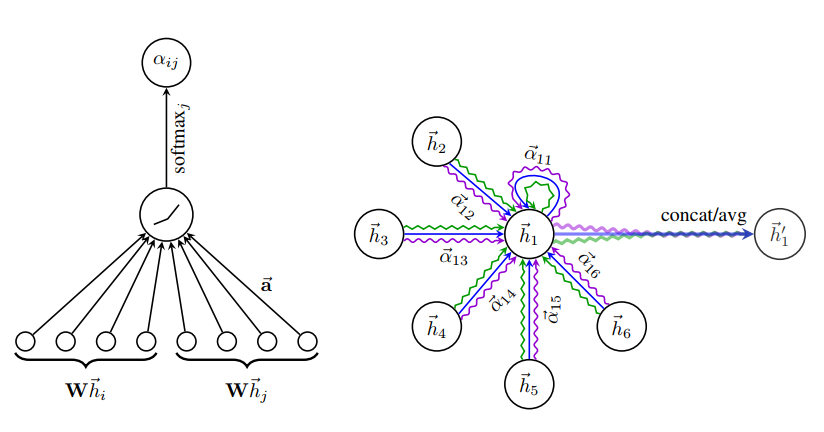
\includegraphics[scale = 1]{Chapter1/Figs/Figure1.png}
	\caption{\textbf{Left}: Cơ chế quan tâm 
			\(a(\textbf{W}\vec{h}_i\|\textbf{W}\vec{h}_j)\)
			được sử dụng bởi mô hình của chúng tôi, được tham số hóa bởi một vectơ trọng số 
			\(\vec{\textbf{a}} \in \mathbb{R}^{2F'}\),
		   áp dụng một hoạt động LeakyReLU. Bên phải: Một minh hoạ của quan tâm đa đầu (với $K = 3$ đầu) bởi nút 1 trên khu vực xung quanh của nó. Các kiểu mũi tên và màu sắc khác nhau đại diện cho các tính toán quan tâm độc lập. Các đặc trưng được tổng hợp từ mỗi đầu được nối tiếp hoặc trung bình để đạt được $\vec{h'_1}$,}
	\label{fig:figure1}
\end{figure}
Áp dụng một hàm phi tuyến, $\sigma$):

\[\vec{h'_i} = \sigma ({\displaystyle \sum_{j \in N_i}} \alpha_{ij}\textbf{W}\vec{h}_i)\]

Để stabilizr quá trình học tự quan tâm, chúng tôi đã tìm thấy mở rộng cơ chế của chúng tôi để sử dụng quan tâm đa đầu có lợi, tương tự như Vaswani et al. (2017). Cụ thể, K cơ chế quan tâm độc lập thực hiện biến đổi của Phương trình 4, và sau đó các đặc trưng của chúng được nối tiếp, dẫn đến biểu diễn đặc trưng đầu ra sau:

\begin{figure} [!ht]
	\centering
	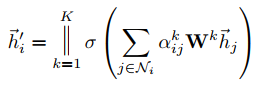
\includegraphics[scale = 0.7]{Chapter1/Figs/ct5.png}
	%\caption{Data Annotation process}
	\label{fig:ct1}
\end{figure}

Trong đó, $\|$ đại diện cho việc nối tiếp, $\alpha_{ij}^k$ là các hệ số quan tâm đã chuẩn hóa được tính bởi cơ chế quan tâm \textit{k}-th ($a^k$), và $\textbf{W}^k$ là ma trận trọng số biến đổi tuyến tính đầu vào tương ứng. Lưu ý rằng, trong tình huống này, kết quả trả về cuối cùng, \textbf{h'}, sẽ bao gồm $KF'$ đặc trưng (thay vì $F'$) cho mỗi nút.

Đặc biệt, nếu chúng ta thực hiện quan tâm đa đầu trên lớp cuối cùng (dự đoán) của mạng, việc nối tiếp không còn hợp lý - thay vào đó, chúng tôi sử dụng trung bình, và hoãn áp dụng nonlinearity cuối cùng (thường là một softmax hoặc sigmoid logistic cho các vấn đề phân loại) cho đến khi đó:

\[
\vec{h'_i} = \sigma (
\frac{1}{K}
{\displaystyle \sum_{k=1}^K}
{\displaystyle \sum_{j \in N_i}} 
\alpha_{ij}^k\textbf{W}^k\vec{h}_i)
\]

Quá trình tập hợp của một lớp quan tâm đồ thị đa đầu được minh họa bởi Hình 1 (bên phải).

% -------------------------------------------------------------------
% Data Annotation
% -------------------------------------------------------------------
\section{So sánh với các nghiên cứu trước}
\label{sec:So sánh với các nghiên cứu trước}
Lớp quan sát đồ thị mô tả trong phần 2.1 trực tiếp giải quyết một số vấn đề xuất hiện trong các phương pháp trước đó về mô hình hóa dữ liệu cấu trúc đồ thị:
	\begin{itemize}
		\item Tính toán hiệu quả: hoạt động của lớp tự quan tâm có thể được đồng bộ hóa trên tất cả các cạnh và tính toán của đặc trưng đầu ra có thể được đồng bộ hóa trên tất cả các nút. Không cần phải tính toán các phép biến đổi ma trận giống như tính toán $eigendecompositions$ hoặc các phép toán ma trận tương tự chi phí cao. Độ phức tạp của một đầu quan tâm GAT tính toán đặc trưng $F'$ có thể biểu diễn dưới dạng $O(|V|F F' + |E|F')$, $F$ là số lượng các đặc trưng đầu vào, $|V|$ và $|E|$ là số lượng nút và cạnh trong đồ thị, tương ứng. Độ phức tạp này tương đương với các phương pháp cơ sở như Mạng Convolutional đồ thị (GCN) (Kipf \& Welling, 2017). Áp dụng nhiều đầu chú ý tăng yêu cầu lưu trữ và tham số lên một yếu tố K, trong khi tính toán của các đầu riêng biệt là hoàn toàn độc lập và có thể song song hóa.
		
		\item Khác với GCNs, mô hình của chúng tôi cho phép (ẩn định) gán sự quan trọng khác nhau cho các nút trong một khu vực giống nhau, cho phép mô hình có khả năng lớn hơn. Ngoài ra, phân tích trọng số chú ý đã học có thể dẫn đến lợi ích trong khả năng hiểu biết, như trong lĩnh vực dịch máy (ví dụ, phân tích chất lượng của Bahdanau et al. (2015))
		
		\item Mechanism attention được áp dụng theo cách chung cho tất cả các cạnh trong đồ thị và do đó không phụ thuộc vào truy cập trước tiên đến cấu trúc đồ thị toàn cầu hoặc (các đặc trưng của) tất cả nút (một hạn chế của nhiều kỹ thuật trước đó). Điều này có nhiều hậu quả mong muốn:
			\begin{itemize}
				\item[-] Không yêu cầu đồ thị phải là không hướng (chúng ta có thể để trống tính toán $ij$ nếu cạnh 
				\(j \longrightarrow i\)
				không tồn tại).
				
				\item[-] Cách tiếp cận của chúng ta cho phép áp dụng trực tiếp cho huấn luyện tại chỗ - bao gồm các nhiệm vụ nơi mô hình được đánh giá trên các đồ thị hoàn toàn chưa từng nhìn thấy trong quá trình huấn luyện.
			\end{itemize}
		
		\item Kỹ thuật chú ý được áp dụng theo cách chung đến tất cả các cạnh trong đồ thị và do đó, nó không phụ thuộc vào truy cập trước tới cấu trúc đồ thị toàn cầu hoặc tính năng của tất cả nút (giới hạn của nhiều kỹ thuật trước đó). Điều này có nhiều kết quả mong muốn: cách tiếp cận mới của Hamilton et al. (2017) lấy mẫu một vùng lưới cố định của mỗi nút để giữ cho chân dung tính toán giống nhau, điều này không cho phép truy cập tới toàn bộ vùng lưới trong quá trình suy diễn. Ngoài ra, kỹ thuật này đạt được một số kết quả mạnh mẽ nhất khi sử dụng chú ý vùng lưới dựa trên LSTM (Hochreiter \& Schmidhuber, 1997). Điều này giả định tồn tại một thứ tự nút liên tục qua các vùng lưới và tác giả đã sửa chữa nó bằng cách truyền vào các dãy ngẫu nhiên được sắp xếp cho LSTM. Cách thức của chúng tôi không gặp phải bất kỳ vấn đề nào của những vấn đề đó - nó hoạt động với toàn bộ khu vực lân cận (với chi phí tính toán biến đổi, vẫn cùng mức với các phương pháp như GCN), và không giả định bất kỳ sắp xếp nào trong nó.
		
		\item GAT có thể được tái cấu trúc thành một trường hợp cụ thể của MoNet (Monti et al., 2016). Cụ thể hơn thiết lập hàm tọa độ giả là $u(x,y) = f(x)\|f(y)$, trong đó $f(x)$ là đặc trưng (có thể được chuyển đổi bằng MLP) của nút x và $\|$ là sự nối tiếp; và hàm trọng lượng là 
		\(\omega_j(u) = softmax(MLP(u))\) 
		(với softmax được thực hiện trên toàn bộ lân cận của một nút), sẽ kiến toán tử patch của MoNet tương tự với chúng tôi. Tuy nhiên, cần lưu ý rằng, so với các phiên bản MoNet đã được xem xét trước đây, mô hình của chúng tôi sử dụng các tính năng nút để tính toán độ tương tự, thay vì các thuộc tính cấu trúc của nút (giả sử biết trước cấu trúc biểu đồ).
		
	\end{itemize}

Chúng tôi đã có thể tạo ra một phiên bản của lớp GAT sử dụng các hoạt dộng ma trận rỗng, giảm độ phức tạp lưu trữ thành tuyến tính trong số lượng nút và cạnh và cho phép thực thiện các mô hình GAT trên các tập dữ liệu đồ thị lớn hơn. Tuy nhiên, khung quản lý xử lý tensor mà chúng tôi sử dụng chỉ hỗ trợ nhân ma trận rỗng cho tensor rank-2, điều này hạn chế khả năng nhóm của lớp như hiện tại đã triển khai (đặc biệt là cho các tập dữ liệu có nhiều đồ thị). Định hướng giải quyết hạn chế này là quan trọng đối với công việc trong tương lai. Tùy thuộc vào tính chính xác của cấp trúc đồ thị, GPU có thể không cung cấp lợi ích hiệu suất lớn so với CPU trong những trường hợp rỗng. Nên chú ý rằng kích thước của “Khung nhìn” của mô hình của chúng tôi được giới hạn bởi độ sâu của mạng (tương tự cho GCN và các mô hình tương tự). Kỹ thuật như kết nối bỏ qua (He et al., 2016) có thể được áp dụng dễ dàng để mở rộng độ sâu, tuy nhiên. Cuối cùng việc lập trình song song cho tất cả các cạnh đồ thị, đặc biệt là theo cách phân tán, có thể gặp nhiều tính toán trùng lặp, vì khu vực lân cận thường rất tương đồng trong các đồ thị quan tâm.












